% !TEX root = ../main.tex
% 本文件由 build-tex.sh 从 28-DSP指南-第28章中译.md 生成，改内容请改 md 后重新生成

\chapter{数字信号处理器}\label{ch-28}

数字信号处理是靠数学运算完成的。相比之下，文字处理之类的程序只是把存储的数据重新排列。这意味着为商务和其他通用用途设计的计算机，并没有针对数字滤波、傅里叶分析这类算法做过优化。数字信号处理器(Digital
Signal
Processor)就是专门为处理数字信号处理任务而设计的微处理器。过去十年里，这类器件增长迅猛，从手机到高端科学仪器，到处都在用。事实上，硬件工程师说''DSP''指的是数字信号处理器，正如算法开发者说''DSP''指的是数字信号处理。本章讨论
DSP 和其他类型的微处理器有什么不同，怎样判断 DSP
是否适合你的应用，以及怎样开始进入这个令人兴奋的新领域。下一章我们会更仔细地看其中一款精巧的产品：Analog
Devices 公司的 SHARC® 系列。

\section{DSP 与其他微处理器有何不同}

20 世纪 60 年代，人们预言人工智能(artificial
intelligence)将彻底改变人类与计算机和其他机器打交道的方式。当时认为到世纪末，机器人会替我们打扫房子，计算机会替我们开车，语音界面会控制信息的存取。这些都没有实现；这些抽象的任务远比预想的复杂，用数字计算机那种一步一步的逻辑很难完成。

不过，过去四十年表明，计算机在两大领域极其能干：(1) 数据操作(data
manipulation)，例如文字处理和数据库管理；(2) 数学计算(mathematical
calculation)，用于科学、工程和数字信号处理。所有微处理器都能做这两类任务，但要造一个同时针对两者都优化的器件很难（也很贵）。硬件设计里有技术上的取舍，比如指令集的规模、中断怎样处理。更重要的是还牵涉市场因素：开发和制造成本、竞争地位、产品寿命等等。笼统地说，这些因素使传统微处理器（如奔腾(Pentium®)）主要面向数据操作。同样，DSP
被设计成执行数字信号处理所需的数学计算。

\begin{figure}[htbp]
\centering
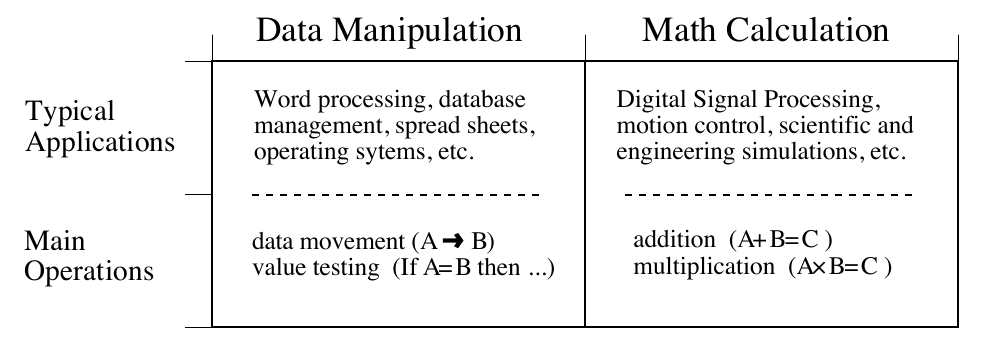
\includegraphics[width=0.821\linewidth,height=0.8\textheight,keepaspectratio]{assets/ch28/fig28-01.png}
\caption*{\textbf{图 28-1　数据操作与数学计算。}
数字计算机适用于两类一般任务：数据操作和数学计算。数据操作以移动数据和检验不等关系为基础，数学计算则使用乘法和加法。
（Data Manipulation = 数据操作，Math Calculation = 数学计算；Typical
Applications =
典型应用：左栏为文字处理、数据库管理、电子表格、操作系统等，右栏为数字信号处理、运动控制、科学与工程仿真等；Main
Operations = 主要运算：左栏为数据移动 (A \dspsym{→} B)、数值检验 (If A=B
then \ldots)，右栏为加法 (A+B=C)、乘法 (A×B=C)。图中 sytems 是 systems
的拼写错误。）}
\end{figure}

图 28-1
列出了这两类任务之间最重要的区别。数据操作涉及信息的存储和排序。以文字处理程序为例，基本任务是存储信息（由操作者键入）、组织信息（剪切粘贴、拼写检查、页面排版等），然后取出信息（例如把文档存到软盘上，或用激光打印机打印出来）。这些任务是靠把数据从一个位置移到另一个位置、以及检验不等关系（A=B、A\textless B
等）来完成的。举个例子，设想把一列单词按字母顺序排序。每个单词用一个 8
位的数表示，即单词首字母的 ASCII
值。按字母排序就是不断调整单词的顺序，直到 ASCII
值从列表开头到结尾一路递增。这可以通过反复执行两个步骤来完成，直到排序完成为止。第一，检验相邻两项是否按字母顺序排列（IF
A\textgreater B THEN
\ldots）；第二，如果这两项没按字母顺序排列，就把它们对调（A\dspsym{⇄}B）。对所有相邻的两项反复执行这两步，列表最终就会排好序。

再举一个例子，想想文字处理软件是怎样打印文档的。计算机不断检测输入设备（鼠标或键盘）上是否出现表示''打印文档''的二进制代码。一旦检测到这个代码，程序就把数据从计算机内存移到打印机。这里还是同样两种基本操作：移动数据和检验不等关系。虽然这类应用偶尔也用到数学，但用得很少，不会明显影响整体的执行速度。

相比之下，大多数 DSP
算法的执行速度几乎完全受限于所需乘法和加法的次数。例如，图 28-2 给出了
FIR 数字滤波器(FIR digital filter)的实现，这是最常见的 DSP
技术。按照标准记法，输入信号记作 x{[} {]}，输出信号记作 y{[}
{]}。我们的任务是计算输出信号中位置 n 处的采样，即 y{[}n{]}。FIR
滤波器的算法是：把输入信号中相应的采样与一组系数（记作
a₀、a₁、a₂、a₃、\dspsym{⋯}）相乘，再把乘积相加。写成公式，y{[}n{]}
这样求出：

\[y[n] = a_0\,x[n] + a_1\,x[n-1] + a_2\,x[n-2] + a_3\,x[n-3] + a_4\,x[n-4] + \cdots\]

这只是在说，输入信号与一个由 a₀、a₁、a₂、a₃、\dspsym{⋯}
组成的滤波器核（即冲激响应）做了卷积。视应用不同，滤波器核里可能只有几个系数，也可能有好几千个。虽然这个算法里也有一些数据传送和不等关系判断，比如记录中间结果和控制循环，但执行时间主要被数学运算占据。

\begin{figure}[htbp]
\centering
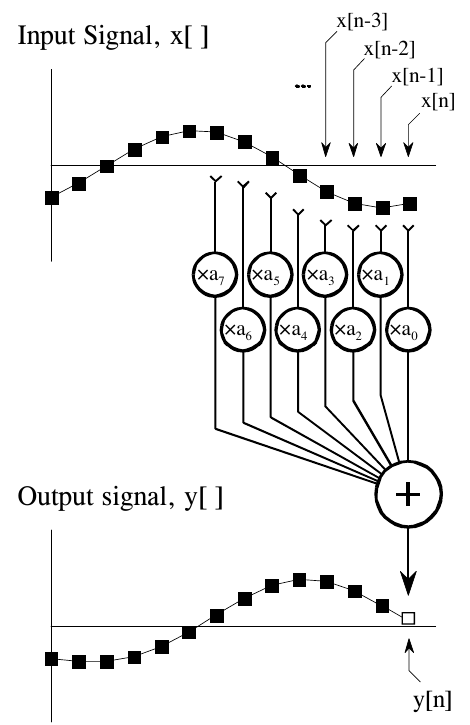
\includegraphics[width=0.392\linewidth,height=0.8\textheight,keepaspectratio]{assets/ch28/fig28-02.png}
\caption*{\textbf{图 28-2　FIR 数字滤波器。} 在 FIR 滤波中，输出信号的每个采样
y{[}n{]}，都是把输入信号的采样
x{[}n{]}、x{[}n−1{]}、x{[}n−2{]}、\dspsym{⋯} 与滤波器核系数
a₀、a₁、a₂、a₃、\dspsym{⋯} 相乘、再把乘积相加得到的。 （Input Signal,
x{[} {]} = 输入信号 x{[} {]}；Output signal, y{[} {]} = 输出信号 y{[}
{]}；圆圈中的 ×a₀～×a₇ 表示乘以对应系数，\dspsym{⊕}
表示相加。原书图注排在图左侧，裁图时已去掉，译文见上。）}
\end{figure}

除了要极快地完成数学计算，DSP
还必须有可预测的执行时间。假设你让台式计算机去做某个任务，比如把一个文字处理文档从一种格式转换成另一种。处理花了十毫秒还是十秒并不要紧；你只需等它做完，再给计算机下一个任务。

相比之下，大多数 DSP
用在处理连续进行、没有明确起止的场合。例如，设想一位工程师在为音频信号设计
DSP 系统，比如助听器。如果数字信号以每秒 20,000 个采样的速率到来，DSP
就必须能持续维持每秒 20,000
个采样的吞吐量。然而，有很重要的理由不让它比需要的更快：速度越高，成本、功耗、设计难度等也越高。因此，准确掌握执行时间，对于选择合适的器件以及能采用的算法都至关重要。

\section{循环缓冲}

数字信号处理器是为快速执行 FIR
滤波器及类似技术而设计的。要理解硬件，先得理解算法。本节详细列出实现一个
FIR 滤波器所需的步骤；下一节我们会看到 DSP
是怎样被设计成尽可能高效地执行这些步骤的。

首先，要区分离线处理(off-line processing)和实时处理(real-time
processing)。在离线处理中，整个输入信号同时存放在计算机里。例如，地球物理学家可能用地震仪记录地震期间的地面运动；震动结束后，再把信息读进计算机做某种分析。离线处理的另一个例子是医学成像，比如计算机断层成像和磁共振成像(MRI)：数据是在病人躺在机器里时采集的，但图像重建可以推迟到以后再做。关键在于，处理程序可以同时拿到全部信息。这在科学研究和工程中很常见，但在消费类产品中并不常见。离线处理是个人计算机和大型机的天地。

在实时处理中，输出信号是在采集输入信号的同时产生的。例如，电话通信、助听器和雷达都需要这样。这些应用必须让信息立即可用，尽管可以有一点点延迟。例如，电话通话中
10
毫秒的延迟，说话人和听话人都察觉不到。同样，雷达信号在显示给操作员之前延迟几秒也无关紧要。实时应用不断重复：输入一个采样，执行算法，输出一个采样。或者，它们也可以输入一组采样，执行算法，再输出一组采样。这就是数字信号处理器的世界。

\begin{figure}[htbp]
\centering
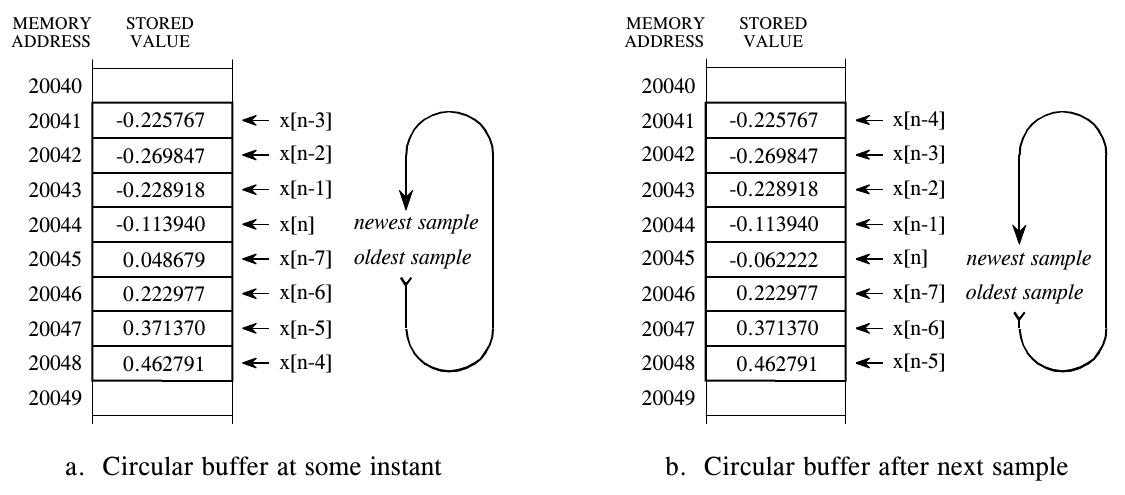
\includegraphics[width=0.938\linewidth,height=0.8\textheight,keepaspectratio]{assets/ch28/fig28-03.png}
\caption*{\textbf{图 28-3　循环缓冲的工作方式。}
循环缓冲用来存储一个不断更新的信号的最新若干个值。本图展示了一个 8
采样的循环缓冲在某一时刻可能的样子 (a)，以及一个采样之后的样子 (b)。
（MEMORY ADDRESS = 内存地址，STORED VALUE = 存储的值；newest sample =
最新的采样，oldest sample = 最旧的采样；a. Circular buffer at some
instant = 某一时刻的循环缓冲，b. Circular buffer after next sample =
下一个采样到来后的循环缓冲。）}
\end{figure}

现在回头看图 28-2，设想这是一个实时实现的 FIR
滤波器。要计算输出采样，我们必须能取到输入中最近的若干个采样。例如，假设这个滤波器用
8 个系数 a₀、a₁、\dspsym{⋯}、a₇，这意味着我们必须知道输入信号最近 8
个采样的值 x{[}n{]}、x{[}n−1{]}、\dspsym{⋯}、x{[}n−7{]}。这 8
个采样必须存放在内存里，并随着新采样的到来不断更新。管理这些存储的采样，最好的办法是什么？答案是循环缓冲(circular
buffering)。

图 28-3 展示了一个 8 采样的循环缓冲。我们把它放在 8
个连续的内存单元里，地址从 20041 到 20048。图 (a) 显示输入的 8
个采样在某个特定时刻可能的存放方式，(b)
显示下一个采样到来之后的变化。循环缓冲的思路是把这个线性数组的末尾和开头接起来：内存单元
20041 被看作紧挨着 20048，就像 20044 紧挨着 20045
一样。用一个指针(pointer)（一个其值为地址的变量）指示最新采样所在的位置，以此来跟踪这个数组。例如，(a)
中指针的值是地址 20044，(b) 中是
20045。新采样到来时，它替换数组中最旧的采样，指针向前移动一个地址。循环缓冲很高效，因为新采样到来时只需改动一个值。

管理一个循环缓冲需要四个参数。第一，要有一个指针指示循环缓冲在内存中的起点（本例中为
20041）。第二，要有一个指针指示数组的终点（例如
20048），或者一个保存其长度的变量（例如
8）。第三，必须指定内存寻址的步长。在图 28-3 中步长是 1，例如：地址
20043 存一个采样，地址 20044
存下一个采样，以此类推。实际情况常常不是这样。例如，寻址可能以字节为单位，而每个采样可能需要两个或四个字节来存放它的值。这时步长就分别要设为
2 或 4。

这三个值确定了循环缓冲的大小和结构，在程序运行期间不会改变。第四个值，即指向最新采样的指针，必须随着每个新采样的到来而修改。换句话说，必须有程序逻辑根据前三个值来控制第四个值如何更新。这个逻辑虽然很简单，但必须非常快。这正是这番讨论的要点：DSP
应当针对循环缓冲的管理进行优化，以获得尽可能高的执行速度。

顺便说一句，循环缓冲在离线处理中也有用。考虑一个输入信号和输出信号都完全存放在内存里的程序。做卷积计算不需要循环缓冲，因为每个采样都能立即取到。然而，许多算法是分级实现的，每两级之间产生一个中间信号。例如，以一串双二阶节(biquad)实现的递归滤波器就是这样工作的。蛮力做法是把每个中间信号的全长都存进内存。循环缓冲提供了另一种选择：只存放当前计算所需的那些中间采样。这样以算法更复杂为代价，减少了所需的内存。重要的观念是：循环缓冲对离线处理有用，对实时应用则至关重要。

现在我们来看，输入信号和系数都用循环缓冲时，实现一个 FIR
滤波器需要哪些步骤。这张清单可能显得琐碎、过于较真------其实不然！高效地处理这些单个任务，正是
DSP 与传统微处理器的区别所在。对每个新采样，都需要执行下面所有步骤：

\textbf{表 28-1　FIR 滤波器的步骤。}

\begin{enumerate}
\def\labelenumi{\arabic{enumi}.}
\tightlist
\item
  用 ADC 获取一个采样；产生一个中断
\item
  检测并处理中断
\item
  把采样移入输入信号的循环缓冲
\item
  更新输入信号循环缓冲的指针
\item
  把累加器清零
\item
  控制循环，遍历每个系数
\item
  从系数的循环缓冲中取出系数
\item
  更新系数循环缓冲的指针
\item
  从输入信号的循环缓冲中取出采样
\item
  更新输入信号循环缓冲的指针
\item
  把系数与采样相乘
\item
  把乘积加到累加器上
\item
  把输出采样（累加器）移到一个暂存缓冲
\item
  把输出采样从暂存缓冲移到 DAC
\end{enumerate}

目标是让这些步骤快速执行。由于第 6～12
步要重复很多次（滤波器的每个系数各一次），需要特别关注这些操作。传统微处理器一般必须串行地（一个接一个地）执行这
14 个步骤，而 DSP
被设计成并行执行它们。在某些情况下，循环内的所有操作（第 6～12
步）可以在一个时钟周期内完成。我们来看看实现这种了不起性能的内部结构。

\section{数字信号处理器的结构}

执行 DSP
算法的最大瓶颈之一，是与内存之间来回传送信息。这既包括数据（比如输入信号的采样和滤波器系数），也包括程序指令（送进程序定序器的二进制代码）。例如，假设我们需要把内存中某处的两个数相乘。为此必须从内存取出三个二进制值：两个被乘数，再加上描述要做什么的程序指令。

图 28-4a
展示了在传统微处理器中，这个看似简单的任务是怎样完成的。这常被称为冯·诺依曼结构(Von
Neumann architecture)，以杰出的美国数学家约翰·冯·诺依曼（John Von
Neumann，1903---1957）命名。冯·诺依曼主导了二十世纪早期许多重要发现背后的数学。他的众多成就包括：提出存储程序计算机的概念、把量子力学的数学形式化，以及参与原子弹的研制。只要是新鲜、激动人心的东西，冯·诺依曼都在场！

如 (a)
所示，冯·诺依曼结构只有一个存储器，和一条在中央处理器(CPU)与存储器之间传送数据的总线。两个数相乘至少需要三个时钟周期，每个周期把三个数中的一个经总线从存储器传到
CPU。我们不计把结果送回存储器的时间，因为假定它留在 CPU
里做进一步处理（比如 FIR
滤波器里的乘积累加）。如果你满足于串行执行所有任务，冯·诺依曼设计就相当令人满意。事实上，今天的大多数计算机都是冯·诺依曼设计。只有在需要非常快的处理、并且愿意为增加的复杂性付出代价时，我们才需要别的结构。

这就引出了 (b) 所示的哈佛结构(Harvard architecture)。它得名于 20 世纪 40
年代在霍华德·艾肯（Howard
Aiken，1900---1973）领导下在哈佛大学所做的工作。如图所示，艾肯坚持把数据和程序指令放在不同的存储器里，各有各的总线。由于两条总线独立工作，程序指令和数据可以同时取出，比单总线设计更快。当今大多数
DSP 都采用这种双总线结构。

图 (c) 展示了更进一步的超级哈佛结构(Super Harvard
Architecture)。这个术语是 Analog Devices 公司创造的，用来描述其
ADSP-2106x 和新的 ADSP-211xx 系列数字信号处理器的内部运作。它们被称为
SHARC® DSP，是 Super Harvard ARChitecture
这个长名字的缩写。其思路是在哈佛结构的基础上增加一些功能来提高吞吐量。SHARC
DSP 在几十个方面做了优化，其中有两点重要到足以画进图
28-4c：指令缓存(instruction cache)和 I/O 控制器(I/O controller)。

\begin{figure}[htbp]
\centering
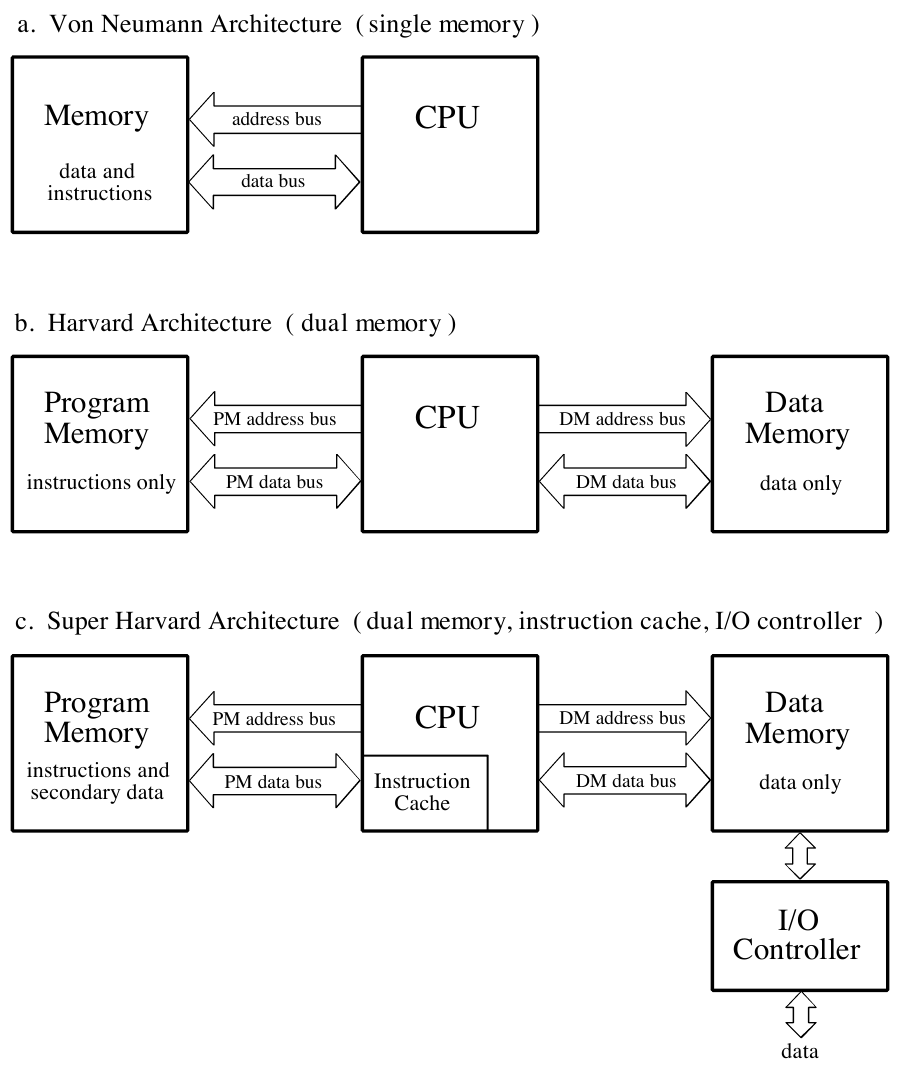
\includegraphics[width=0.754\linewidth,height=0.8\textheight,keepaspectratio]{assets/ch28/fig28-04.png}
\caption*{\textbf{图 28-4　微处理器结构。}
冯·诺依曼结构用一个存储器同时存放数据和指令。相比之下，哈佛结构用不同的存储器分别存放数据和指令，速度更高。超级哈佛结构在哈佛设计的基础上增加了指令缓存和专用的
I/O 控制器。 （a. Von Neumann Architecture (single memory) =
冯·诺依曼结构（单存储器）；b. Harvard Architecture (dual memory) =
哈佛结构（双存储器）；c.~Super Harvard Architecture (dual memory,
instruction cache, I/O controller) =
超级哈佛结构（双存储器、指令缓存、I/O 控制器）。Memory = 存储器，data
and instructions = 数据和指令；Program Memory = 程序存储器，instructions
only = 只存指令，instructions and secondary data = 指令和次要数据；Data
Memory = 数据存储器，data only = 只存数据；address bus / data bus =
地址总线 / 数据总线，PM = 程序存储器，DM = 数据存储器；Instruction Cache
= 指令缓存；I/O Controller = I/O
控制器。原书图注排在图左下，裁图时已去掉，译文见上。）}
\end{figure}

先看指令缓存怎样提升哈佛结构的性能。基本哈佛设计的一个短板是：数据存储器总线比程序存储器总线忙。两个数相乘时，两个二进制值（被乘数）必须经数据存储器总线传送，而程序存储器总线只传送一个二进制值（程序指令）。为改善这种状况，我们先把一部分''数据''挪到程序存储器里。例如，可以把滤波器系数放在程序存储器中，而输入信号仍留在数据存储器中。（图中把这些挪过去的数据称为''次要数据(secondary
data)``。）乍一看这并没有改善情况：现在数据存储器总线要传一个值（输入信号采样），程序存储器总线却要传两个值（程序指令和系数）。事实上，如果执行的是随机的指令，情况一点也不会更好。

然而，DSP 算法一般把大部分执行时间花在循环里，比如表 28-1 的第 6～12
条指令。这意味着同一组程序指令会不断地从程序存储器送到
CPU。超级哈佛结构利用了这一点，在 CPU
中加入了指令缓存。这是一块小存储器，存放最近的约 32
条程序指令。第一次执行循环时，程序指令必须经程序存储器总线传送，由于和同样要走这条路的系数冲突，速度会慢一些。然而在后续的循环执行中，程序指令可以从指令缓存中取出。这意味着所有从存储器到
CPU
的信息传送都可以在一个周期内完成：输入信号的采样经数据存储器总线传来，系数经程序存储器总线传来，程序指令则来自指令缓存。用行话说，这种高效的数据传送叫做高存储器访问带宽(high
memory-access bandwidth)。

图 28-5 更详细地展示了 SHARC 结构，画出了连接到数据存储器的 I/O
控制器。信号就是从这里进出系统的。例如，SHARC DSP
同时提供串行和并行通信端口，都是极高速的连接。例如在 40 MHz
时钟下，有两个各以 40 Mbit/s 工作的串行端口，六个并行端口则每个提供 40
Mbyte/s 的数据传输。六个并行端口同时使用时，数据传输率高达惊人的 240
Mbyte/s。

这快得足以在短短 2
毫秒内传完本书的全部文字！同样重要的是，专用硬件允许这些数据流直接传进存储器（即直接存储器访问(Direct
Memory Access，DMA)），而不必经过 CPU 的寄存器。换句话说，我们清单上的第
1 项和第 14 项任务与其他任务独立、同时进行，不会占用 CPU
的周期。主总线（程序存储器总线和数据存储器总线）也可以从芯片外部访问，为片外存储器和外设提供了额外的接口。这使得
SHARC DSP 可以使用 4 G 字（16 GB）的存储器，对 32 位数据以 40 M
字/秒（160 MB/s）的速率访问。哇！

这种高速 I/O 是 DSP
的一个关键特征。压倒一切的目标是：在下一个采样到来之前，把数据送进来、做完数学运算、把数据送出去。其余一切都是次要的。有些
DSP 片上带有模数和数模转换器，这一特性叫做混合信号(mixed
signal)。不过，所有 DSP 都能通过串行或并行端口与外部转换器连接。

现在看看 CPU 内部。图的顶部有两个标着数据地址发生器(Data Address
Generator，DAG)的方框，两个存储器各一个。它们控制送往程序存储器和数据存储器的地址，指定信息从哪里读出或写到哪里。在较简单的微处理器中，这项任务是程序定序器固有的一部分，对程序员来说相当透明。然而，DSP
是为使用循环缓冲而设计的，额外的硬件能高效地管理循环缓冲，从中获益。这样就不必耗费宝贵的
CPU 时钟周期去跟踪数据是怎样存放的。例如，在 SHARC DSP 中，两个 DAG
各自能控制 8 个循环缓冲。这意味着每个 DAG 保存 32 个变量（每个缓冲 4
个），外加所需的逻辑。

为什么要这么多循环缓冲？有些 DSP 算法最好分级执行。例如，IIR
滤波器以双二阶节（一个含两个极点和至多两个零点的级）级联的方式实现时更稳定。多级就需要多个循环缓冲才能运行得最快。SHARC
DSP 中的 DAG 还被设计成能高效地执行快速傅里叶变换。在这种模式下，DAG
被配置成向循环缓冲生成位反转地址(bit-reversed address)，这是 FFT
算法必需的一部分。此外，循环缓冲多了，DSP
代码的生成会大为简化------对人类程序员和 C
之类的高级语言编译器都是如此。

CPU 的数据寄存器部分，用法与传统微处理器相同。ADSP-2106x SHARC DSP 中有
16 个通用寄存器，每个 40
位。它们可以保存中间计算结果、为数学处理器准备数据、充当数据传送的缓冲、保存程序控制用的标志等等。需要的话，这些寄存器也可以用来控制循环和计数器；不过
SHARC DSP 有额外的硬件寄存器来完成其中许多功能。

数学处理分成三个部分：乘法器(multiplier)、算术逻辑单元(arithmetic logic
unit，ALU)和桶形移位器(barrel
shifter)。乘法器从两个寄存器取值，相乘后把结果放进另一个寄存器。ALU
执行加法、减法、绝对值、逻辑运算（AND、OR、XOR、NOT）、定点与浮点格式之间的转换以及类似的功能。基本的二进制操作由桶形移位器完成，例如移位、循环移位、提取和存入位段等。SHARC
系列的一个强大特性是乘法器和 ALU 可以并行访问。在一个时钟周期内，寄存器
0～7 的数据可以送给乘法器，寄存器 8～15 的数据可以送给
ALU，两个结果再送回 16 个寄存器中的任意一个。

\begin{figure}[htbp]
\centering
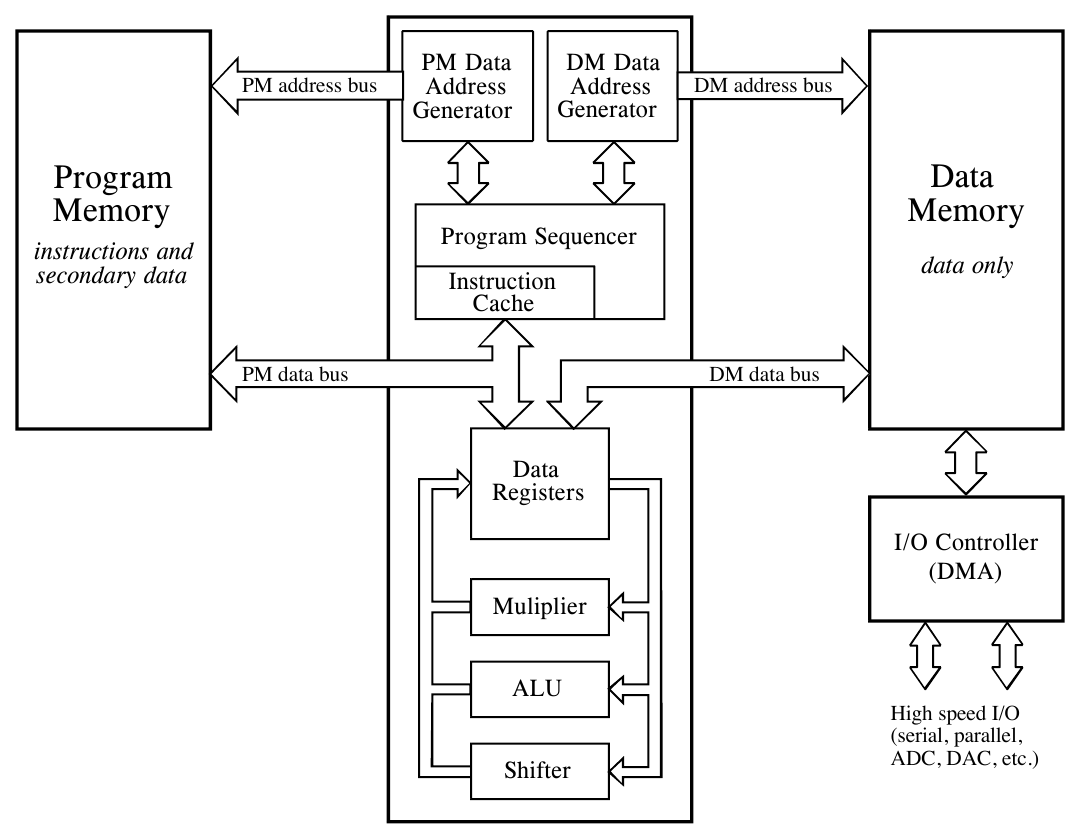
\includegraphics[width=0.900\linewidth,height=0.8\textheight,keepaspectratio]{assets/ch28/fig28-05.png}
\caption*{\textbf{图 28-5　典型的 DSP 结构。}
数字信号处理器被设计成并行地执行任务。这张简化图画的是 Analog Devices 的
SHARC DSP。把这个结构与实现 FIR 滤波器所需的任务（列在表 28-1
中）对照一下：循环内的所有步骤都可以在一个时钟周期内执行。 （Program
Memory = 程序存储器，instructions and secondary data =
指令和次要数据；Data Memory = 数据存储器，data only = 只存数据；PM / DM
Data Address Generator = 程序 / 数据存储器的数据地址发生器；Program
Sequencer = 程序定序器，Instruction Cache = 指令缓存；Data Registers =
数据寄存器，Muliplier = 乘法器（原书拼错，应为 Multiplier），ALU =
算术逻辑单元，Shifter = 移位器；I/O Controller (DMA) = I/O
控制器（DMA）；High speed I/O (serial, parallel, ADC, DAC, etc.) = 高速
I/O（串行、并行、ADC、DAC 等）。）}
\end{figure}

SHARC
系列结构中还有许多重要特性没画在这张简化图里。例如，乘法器内置了一个 80
位的累加器，以减少多次定点运算带来的舍入误差。另一个有趣的特性是：CPU
的所有关键寄存器都配有影子寄存器(shadow
register)。这些是可以在一个时钟周期内与原寄存器互换的副本，用于快速上下文切换(context
switching)，即快速响应中断的能力。在传统微处理器中，发生中断时，必须先保存所有内部数据才能处理中断，这通常要把所有占用的寄存器一个一个地压入堆栈。相比之下，SHARC
系列处理中断时，在一个时钟周期内把内部数据移进影子寄存器；中断程序结束后，寄存器又同样快速地恢复。这一特性使我们清单上的第
4 步（处理''采样就绪''中断）能被非常快速高效地处理。

\begin{quote}
\textbf{译注：} 按表 28-1，``检测并处理中断''是第 2 步，第 4
步是更新输入缓冲的指针，原文此处步号应为 2。
\end{quote}

现在来到这个结构最关键的性能：循环内的操作（表 28-1 的第 6～12
步）有多少能同时执行。由于高度并行，SHARC DSP
可以同时执行所有这些任务。具体地说，在一个时钟周期内，它可以执行一次乘法（第
11 步）、一次加法（第 12 步）、两次数据移动（第 7 和第 9
步）、更新两个循环缓冲指针（第 8 和第 10 步），以及控制循环（第 6
步）。循环的开始和结束会有额外的时钟周期（第 3、4、5 和 13
步，外加把初始值放到位）；不过这些任务也处理得非常高效。如果循环执行的次数不止几次，这些开销就可以忽略。例如，假设你用
100 个系数写了一个高效的 FIR 滤波器程序，可以预期每个采样需要约 105 到
110 个时钟周期（即 100
次系数循环加上开销）。这非常了不起；传统微处理器执行这个算法需要好几千个时钟周期。

\section{定点与浮点}

数字信号处理可以分为两类：定点(fixed point)和浮点(floating
point)。这指的是器件内部存储和处理数字所用的格式。定点 DSP 通常用至少 16
位表示每个数，不过也可以用别的长度。例如，摩托罗拉生产一个使用 24
位的定点 DSP 系列。这 \(2^{16} = 65{,}536\)
种可能的位模式有四种常见的表示数的方法。无符号整数(unsigned
integer)中，存储的数可以取 0 到 65,535
之间的任何整数值。类似地，有符号整数(signed
integer)用二进制补码使范围包括负数，从 −32,768 到
32,767。无符号小数(unsigned fraction)表示法把 65,536 个电平均匀地分布在
0 和 1 之间。最后，有符号小数(signed fraction)格式允许负数，在 −1 和 1
之间等间隔分布。

相比之下，浮点 DSP 通常用至少 32
位存储每个值。这样得到的位模式比定点多得多，准确地说是
\(2^{32} = 4{,}294{,}967{,}296\)
个。浮点表示法的一个关键特点是：所表示的数不是均匀分布的。在最常见的格式（ANSI/IEEE
Std. 754-1985）中，最大和最小的数分别是 ±3.4×10³⁸ 和
±1.2×10⁻³⁸。所表示的值在这两个极端之间不等间隔分布，使得任意两个相邻数之间的间隙约为数值本身的千万分之一。这一点很重要，因为它在大数之间留下大间隙，在小数之间留下小间隙。浮点表示法在第
4 章中有更详细的讨论。

所有浮点 DSP 也都能处理定点数，这对实现计数器、循环以及来自 ADC、送往
DAC
的信号是必需的。然而，这并不意味着定点运算会和浮点运算执行得一样快；这取决于内部结构。例如，SHARC
DSP 对浮点和定点运算都做了优化，执行起来效率相同。因此，SHARC
器件常被称为''32 位 DSP''，而不只是''浮点 DSP''。

\begin{figure}[htbp]
\centering
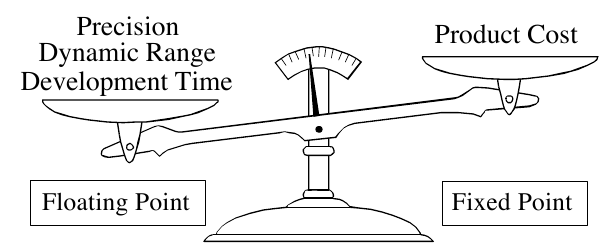
\includegraphics[width=0.508\linewidth,height=0.8\textheight,keepaspectratio]{assets/ch28/fig28-06.png}
\caption*{\textbf{图 28-6　定点与浮点。} 定点 DSP
一般更便宜，而浮点器件精度更好、动态范围更大、开发周期更短。
（天平左盘：Precision = 精度，Dynamic Range = 动态范围，Development Time
= 开发时间，对应 Floating Point = 浮点；右盘：Product Cost =
产品成本，对应 Fixed Point =
定点。原书图注排在图左侧，裁图时已去掉，译文见上。）}
\end{figure}

图 28-6 说明了定点和浮点 DSP 之间的主要取舍。在第 3
章中我们强调过，在通用计算机里定点运算比浮点运算快得多。然而在 DSP
中，两者速度大致相同，这是硬件针对数学运算高度优化的结果。浮点 DSP
的内部结构比定点器件复杂：所有寄存器和数据总线都必须是 32 位宽而不只是
16 位；乘法器和 ALU
必须能快速执行浮点运算；指令集必须更大（以便同时处理浮点数和定点数）；等等。浮点（32
位）比定点（16
位）精度更好、动态范围更大。此外，浮点程序的开发周期往往更短，因为程序员一般不必操心溢出、下溢和舍入误差之类的问题。

\begin{quote}
\textbf{译注：} 定点与浮点运算速度的比较（表 4-6 等）实际在第 4 章''DSP
软件''中，原文''第 3 章''疑为笔误。后文''详见第 3
章''讲累积量化噪声，同样以第 4 章为准。
\end{quote}

另一方面，定点 DSP
传统上比浮点器件便宜。没有什么比电子产品的价格变得更快了；你在书里找到的任何价格在付印前就已过时。尽管如此，成本是理解
DSP 如何演进的关键因素，我们需要给你一个大致的概念。本书在 1999
年完成时，定点 DSP 的售价在 5 美元到 100 美元之间，浮点器件则在 10
美元到 300
美元之间。这种价格差异可以看作两类器件相对复杂度的一个度量。如果你想知道今天的价格，就得今天去查。

现在把注意力转向性能：32 位浮点系统能做到哪些 16
位定点做不到的事？答案是信噪比(signal-to-noise ratio)。假设我们以 32
位浮点格式存储一个数。如前所述，这个数与相邻数之间的间隙约为数值本身的千万分之一。要存储这个数，必须向上或向下舍入，最多舍入半个间隙。换句话说，每次以浮点表示法存储一个数，就给信号添加了噪声。

一个数以 16
位定点值存储时也会发生同样的事，只是添加的噪声要糟得多。这是因为相邻数之间的间隙大得多。例如，假设我们把数
10,000 存为有符号整数（范围从 −32,768 到
32,767），数之间的间隙是所存数值的万分之一。如果要存的是
1000，间隙就是数值的千分之一。

信号中的噪声通常用标准差来表示，这在第 2
章中详细讨论过。在这里，重要的事实是：这种量化噪声的标准差约为间隙大小的三分之一。这意味着存储浮点数时的信噪比约为三千万比一，而定点数只有约一万比一。换句话说，浮点的量化噪声大约比定点小
30,000 倍。

这引出了 DSP 与传统微处理器的一个重要区别。假设我们用定点实现一个 FIR
滤波器：遍历每个系数，乘以输入信号中相应的采样，再把乘积加到累加器上。问题来了。在传统微处理器中，这个累加器只是又一个
16
位定点变量。为避免溢出，我们需要对相加的值进行缩放，每一步都会相应地添加量化噪声。最坏情况下，这些量化噪声会简单地累加，大大降低系统的信噪比。例如，在一个
500 系数的 FIR 滤波器中，每个输出采样上的噪声可能是每个输入采样上噪声的
500
倍。一万比一的信噪比就跌到了糟糕透顶的二十比一。虽然这是个极端情况，但它说明了要点：对每个采样执行很多次运算时，情况很糟，真的很糟。详见第
3 章。

DSP 用扩展精度累加器(extended precision
accumulator)来解决这个问题。这是一个特殊的寄存器，位数是其他存储单元的
2～3 倍。例如，在 16 位 DSP 中它可能有 32 到 40 位，而在 SHARC DSP
中，定点用的累加器有 80
位。这么大的扩展范围几乎消除了累加过程中的舍入噪声。唯一的舍入误差发生在累加器被缩放并存回
16
位存储器的时候。这个策略效果很好，尽管它确实限制了某些算法的实现方式。相比之下，浮点的量化噪声低到通常不需要这些技巧。

除了量化噪声更低，浮点系统上开发算法也更容易。大多数 DSP
技术都基于反复的乘法和加法。在定点中，每次运算之后都要考虑溢出或下溢的可能。程序员需要时刻了解数的幅度、量化误差是怎样累积的、需要做什么缩放。相比之下，浮点中不会出现这些问题；数自己会照顾好自己（极少数情况除外）。

为了让你更好地理解这个问题，图 28-7 给出了 SHARC
用户手册中的一张表，它描述了定点和浮点格式下执行乘法的各种方式。先看浮点数怎样相乘：只有一种方式！那就是
Fn = Fx * Fy，其中 Fn、Fx 和 Fy 是 16
个数据寄存器中的任意一个。简单得不能再简单了。相比之下，看看定点乘法所有可能的指令。这许多选项都是为了高效处理舍入、缩放和格式问题。

\begin{figure}[htbp]
\centering
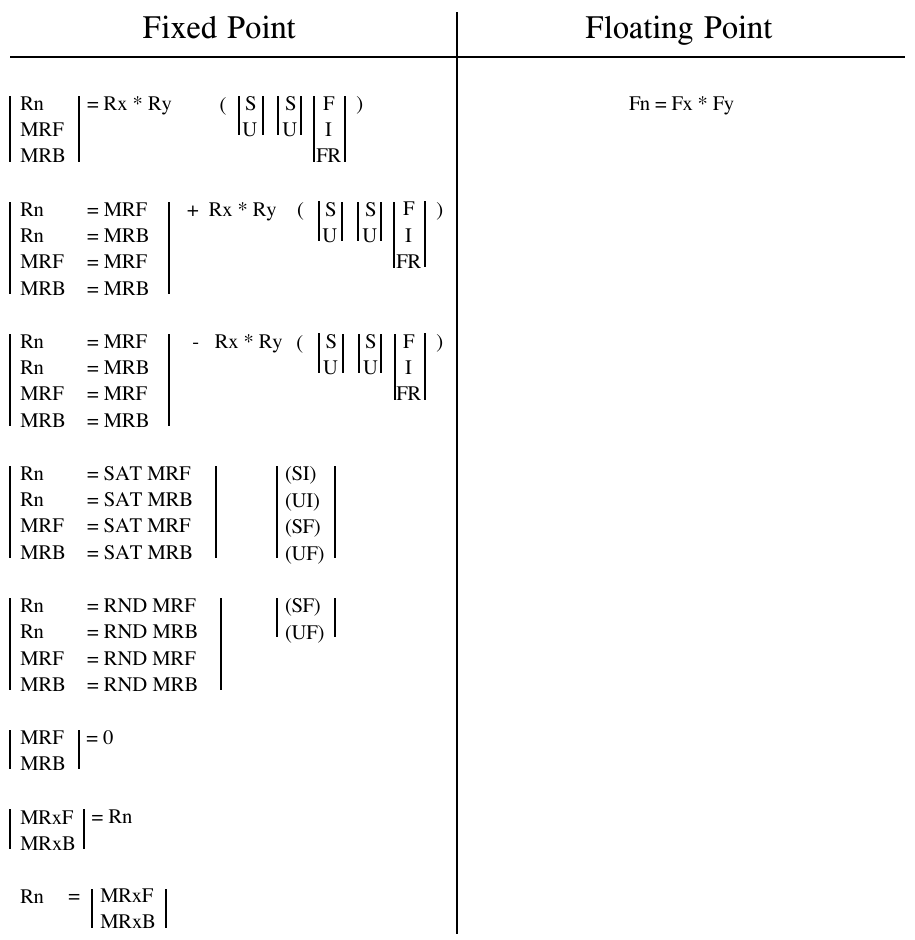
\includegraphics[width=0.762\linewidth,height=0.8\textheight,keepaspectratio]{assets/ch28/fig28-07.png}
\caption*{\textbf{图 28-7　定点与浮点指令。} 这些是 SHARC DSP
中使用的乘法指令。浮点只需一条指令，而定点需要许多选项。各选项的解释见正文。
（Fixed Point = 定点，Floating Point = 浮点。）}
\end{figure}

在图 28-7 中，Rn、Rx 和 Ry 指 16 个数据寄存器中的任意一个，MRF 和 MRB 是
80
位累加器。竖线表示可选项。例如，表左上角那一项意味着下面这些都是合法指令：Rn
= Rx * Ry、MRF = Rx * Ry 和 MRB = Rx *
Ry。换句话说，任意两个寄存器的值都可以相乘，结果放进另一个寄存器或某个扩展精度累加器中。这张表还表明，数可以是有符号的或无符号的（S
或 U），可以是小数或整数（F 或 I）。RND 和 SAT
选项是控制舍入和寄存器溢出的方法。

表中还有其他细节和选项，但对我们眼下的讨论并不重要。重要的观念是：定点程序员必须掌握几十种方式来完成乘法这个非常基本的任务。相比之下，浮点程序员可以把时间集中在算法上。

在定点和浮点之间有这些取舍，你该怎样选择？下面是一些要考虑的事情。第一，看
ADC 和 DAC 用多少位。在许多应用中，每采样 12～14
位是选择定点还是浮点的分界线。例如，电视和其他视频信号一般用 8 位 ADC 和
DAC，定点的精度就够了。相比之下，专业音频应用的采样位数可高达 20 或 24
位，几乎肯定需要浮点来容纳很大的动态范围。

接下来要看所运行算法的复杂度。如果比较简单，就考虑定点；如果比较复杂，就考虑浮点。例如，FIR
滤波和其他时域运算只需要几十行代码，适合定点。相比之下，频域算法（如频谱分析和
FFT
卷积）非常繁琐，编程可能难得多。虽然它们也能用定点写，但用浮点的话开发时间会大大缩短。

最后，想想钱：产品成本有多重要，开发成本又有多重要？选择定点，产品成本会降低，但由于算法更难，开发成本可能更高。反过来，浮点一般会让开发周期更快、更便宜，但最终产品更贵。

\begin{figure}[htbp]
\centering
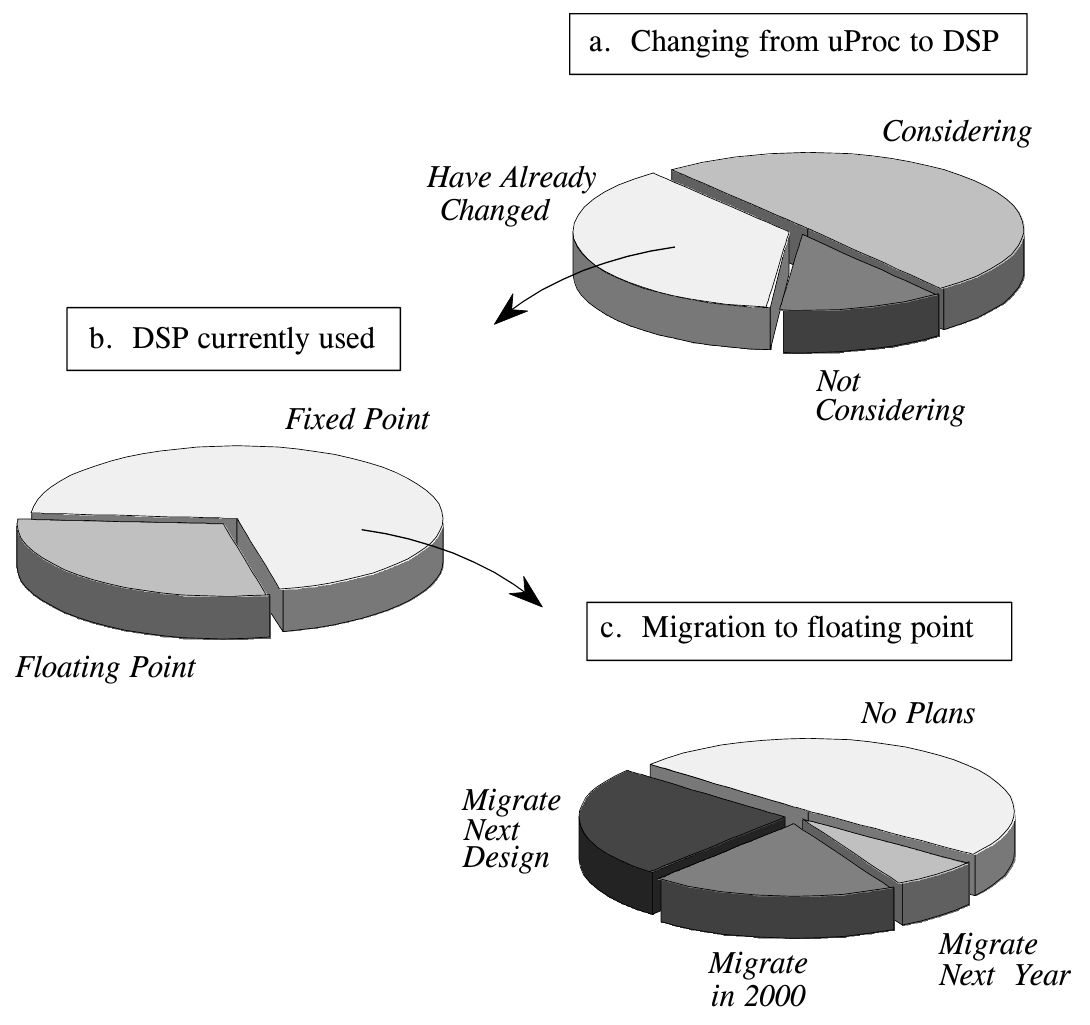
\includegraphics[width=0.908\linewidth,height=0.8\textheight,keepaspectratio]{assets/ch28/fig28-08.png}
\caption*{\textbf{图 28-8　DSP 的主要趋势。} 如 (a) 所示，约 38\%
的嵌入式设计者已经从传统微处理器转向 DSP，另有 49\% 正在考虑转换。在 (b)
中，使用定点 DSP 的工程师约为使用浮点 DSP
的两倍，这主要是由必须采用低成本电子器件的消费类产品（如手机）推动的。然而，如
(c) 所示，浮点是增长最快的部分；目前使用 16
位器件的工程师中，超过一半计划迁移到浮点 DSP。 （a. Changing from uProc
to DSP = 从微处理器转向 DSP：Have Already Changed =
已经转换，Considering = 正在考虑，Not Considering = 不考虑；b. DSP
currently used = 目前使用的 DSP：Fixed Point = 定点，Floating Point =
浮点；c.~Migration to floating point = 向浮点迁移：No Plans =
没有计划，Migrate Next Design = 下一个设计迁移，Migrate in 2000 = 2000
年迁移，Migrate Next Year = 明年迁移。）}
\end{figure}

图 28-8 展示了 DSP 的一些主要趋势。图 (a)
说明了数字信号处理器对嵌入式市场的影响。嵌入式应用是指用微处理器直接操作和控制某个更大系统的应用，比如手机、微波炉或汽车仪表盘。这类器件常被称为''微控制器(microcontroller)``，以区别于个人计算机中使用的微处理器。如
(a) 所示，约 38\% 的嵌入式设计者已经开始使用 DSP，另有 49\%
正在考虑转换。DSP 的高吞吐量和计算能力常常使它成为嵌入式设计的理想选择。

如 (b) 所示，目前使用定点 DSP 的工程师约为使用浮点 DSP
的两倍。不过，这在很大程度上取决于应用。定点在电子器件成本必须压得很低的、竞争激烈的消费类产品中更流行。手机就是一个好例子。当你要和别人竞争、卖出几百万件产品时，区区几美元的成本差异就可能决定成败。相比之下，在需要更高性能、成本不重要的场合，浮点更常见。例如，假设你在设计一个医学成像系统，比如计算机断层扫描仪。这个型号总共只会卖出几百台，每台售价几十万美元。对这种应用来说，DSP
的成本微不足道，性能却至关重要。尽管使用的定点 DSP
数量更多，浮点市场却是增长最快的部分。如 (c) 所示，使用 16
位器件的工程师中超过一半计划在不久的将来迁移到浮点。

在结束这个话题之前，我们要再次强调：浮点和定点通常分别使用 32 位和 16
位，但并非总是如此。例如，SHARC 系列可以用 32
位定点表示数，这种模式在数字音频应用中很常见。这使得 2³²
个量化电平均匀分布在一个相对较小的范围内，比如 −1 到 1
之间。相比之下，浮点表示法把 2³²
个量化电平按对数分布在一个巨大的范围内，通常是 ±3.4×10³⁸。这使 32
位定点有更好的精度(precision)，也就是说，任何一个采样上的量化误差都更小。然而，32
位浮点有更大的动态范围(dynamic
range)，也就是说，能表示的最大数和最小数之间的差别更大。

\section{C 与汇编}

DSP 的编程语言和其他科学、工程应用一样，通常是汇编或
C。用汇编写的程序执行得更快，而用 C
写的程序更容易开发和维护。在传统应用中（比如在个人计算机和大型机上运行的程序），C
几乎总是首选。即使用到汇编，也仅限于必须以最快速度运行的短小子程序。图
28-9a 用图形表示了这一点：每有一个用汇编的传统程序员，就有大约十个用 C
的。

然而，DSP
程序在两个重要方面不同于传统软件任务。第一，程序通常短得多，比如一百行对一万行。第二，执行速度往往是应用的关键部分。毕竟，人们用
DSP
的首要原因就是它惊人的速度。这两个因素促使许多软件工程师在给数字信号处理器编程时从
C 转向汇编。(b) 说明了这一点：DSP 程序员中用汇编的几乎和用 C 的一样多。

图 (c) 更进一步，看的是 DSP 产品创造的收入。用 C 编程的 DSP
每挣一美元，用汇编编程的 DSP
就挣两美元。原因很简单：赚钱靠的是胜过竞争对手。纯粹从性能的角度看（比如执行速度和制造成本），汇编几乎总比
C 有优势。例如，C
代码通常比汇编需要更大的存储器，导致硬件更贵。然而，DSP
市场在不断变化。随着市场增长，厂商会设计出针对 C 编程优化的 DSP
来应对。例如，有大量通用寄存器和统一存储空间时，C
的效率会高得多。这些未来的改进会缩小 C 与汇编之间的执行时间差距，让 C
能用于更多应用。

\begin{figure}[htbp]
\centering
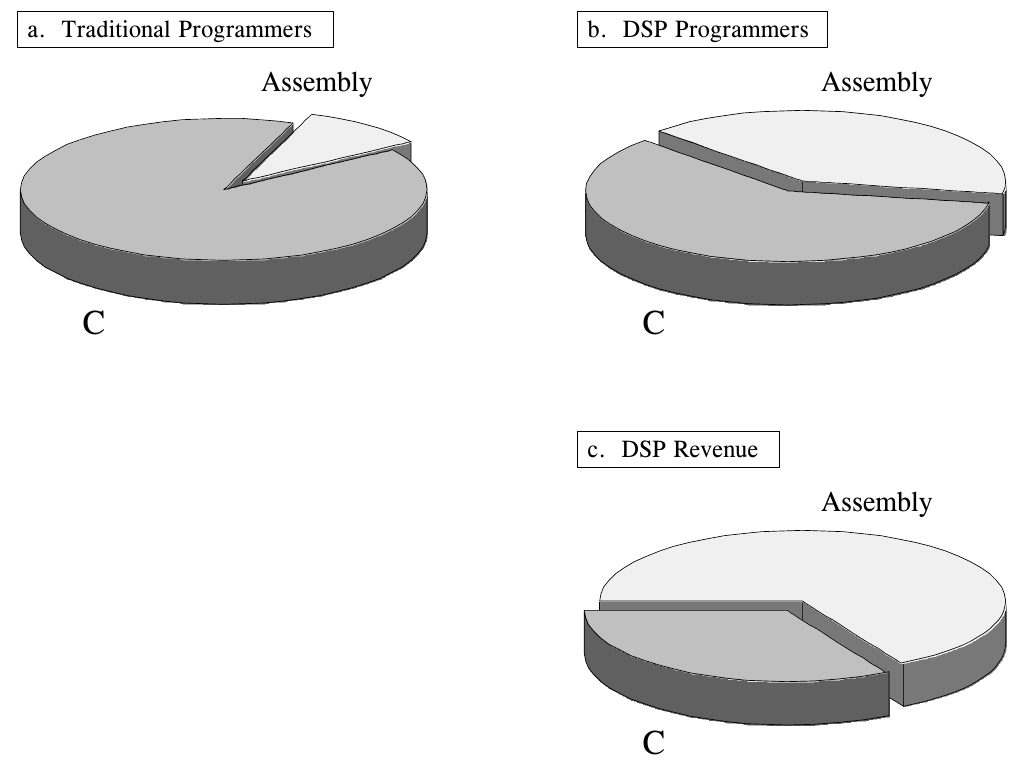
\includegraphics[width=0.858\linewidth,height=0.8\textheight,keepaspectratio]{assets/ch28/fig28-09.png}
\caption*{\textbf{图 28-9　用 C 编程与用汇编编程。} 如 (a)
所示，传统程序员（如在个人计算机和大型机上工作的程序员）中只有约 10\%
使用汇编。然而，如 (b) 所示，汇编在数字信号处理器中要常见得多，这是因为
DSP 程序必须运行得尽可能快，而且通常很短。图 (c)
表明，在创造高收入的产品中，汇编更为常见。 （a. Traditional Programmers
= 传统程序员；b. DSP Programmers = DSP 程序员；c.~DSP Revenue = DSP
收入；Assembly = 汇编，C = C
语言。原书图注排在图左侧，裁图时已去掉，译文见上。）}
\end{figure}

为了更好地理解在 C
和汇编之间的抉择，我们来看一个分别用两种语言编写的典型 DSP
任务。我们用的例子是计算两个数组 x{[} {]} 和 y{[} {]} 的点积(dot
product)。这是一个简单的数学运算：把一个数组中的每个系数乘以另一个数组中对应的系数，再把乘积相加，即
\(x[0]\times y[0] + x[1]\times y[1] + x[2]\times y[2] + \cdots\)。这应该看着很眼熟；它正是
FIR
滤波器中的基本运算。也就是说，输出信号的每个采样，都是把输入信号中存储的采样（在一个数组里）乘以滤波器系数（在另一个数组里），再把乘积相加得到的。

表 28-2 展示了点积在 C 程序中是怎样计算的。在第 001～004
行，我们把两个数组 x{[} {]} 和 y{[} {]} 定义为 20 个元素长，还定义了
result，即程序结束时保存点积计算结果的变量。第 011 行控制计算所需的 20
次循环，用变量 n 作循环计数器。循环中唯一的语句是第 012
行，它把两个数组中对应的系数相乘，再把乘积加到累加器变量 s
上。（如果你不熟悉 C，语句 \texttt{s\ +=\ x{[}n{]}*y{[}n{]}} 的意思和
\texttt{s\ =\ s\ +\ x{[}n{]}*y{[}n{]}} 相同。）循环结束后，第 013
行把累加器 s 中的值传给输出变量 result。

\textbf{表 28-2　用 C 计算点积。} 这个程序计算两个数组 x{[} {]} 和 y{[}
{]} 的点积，并把结果存入变量 result。

\begin{Shaded}
\begin{Highlighting}[]
\BaseNTok{001}\NormalTok{   \#define LEN }\DecValTok{20}
\BaseNTok{002}     \DataTypeTok{float}\NormalTok{ dm x}\OperatorTok{[}\NormalTok{LEN}\OperatorTok{];}
\BaseNTok{003}     \DataTypeTok{float}\NormalTok{ pm y}\OperatorTok{[}\NormalTok{LEN}\OperatorTok{];}
\BaseNTok{004}     \DataTypeTok{float}\NormalTok{ result}\OperatorTok{;}
\BaseNTok{005}
\BaseNTok{006}\NormalTok{   main}\OperatorTok{()}
\BaseNTok{007}
\BaseNTok{00}\ErrorTok{8}   \OperatorTok{\{}
\BaseNTok{00}\ErrorTok{9}     \DataTypeTok{int}\NormalTok{ n}\OperatorTok{;}
\BaseNTok{010}     \DataTypeTok{float}\NormalTok{ s}\OperatorTok{;}
\BaseNTok{011}     \ControlFlowTok{for} \OperatorTok{(}\NormalTok{n}\OperatorTok{=}\DecValTok{0}\OperatorTok{;}\NormalTok{n}\OperatorTok{\textless{}}\NormalTok{LEN}\OperatorTok{;}\NormalTok{n}\OperatorTok{++)}
\BaseNTok{012}\NormalTok{       s }\OperatorTok{+=}\NormalTok{ x}\OperatorTok{[}\NormalTok{n}\OperatorTok{]*}\NormalTok{y}\OperatorTok{[}\NormalTok{n}\OperatorTok{];}
\BaseNTok{013}\NormalTok{     result }\OperatorTok{=}\NormalTok{ s}
\BaseNTok{014}   \OperatorTok{\}}
\end{Highlighting}
\end{Shaded}

\begin{quote}
\textbf{译注：} 照原样，这段程序有两处问题：第 010 行的 s 没有初始化为
0（应写 \texttt{float\ s\ =\ 0;}），第 013 行行末漏了分号。另外
\texttt{dm}、\texttt{pm} 是 SHARC 的 C
编译器扩展的关键字，指定数组放在数据存储器还是程序存储器，标准 C
编译器不认识。原书表注里的 progam 是 program 的拼写错误。
\end{quote}

使用高级语言（如 C、Fortran 或
Basic）的一个关键好处是：程序员不必了解所用微处理器的结构，这方面的知识交给了编译器。例如，这个短短的
C 程序用到了几个变量：n、s、result，以及数组 x{[} {]} 和 y{[}
{]}。所有这些变量都必须在硬件中分配一个''家''来保存它们的值。视微处理器而定，这些存储位置可以是通用数据寄存器、主存储器中的单元，或专门用于特定功能的特殊寄存器。然而，写高级语言程序的人对这种存储管理几乎一无所知；这项任务被委托给了编写编译器的软件工程师。问题是，这两个人从未见过面；他们只通过一套预先定好的规则交流。高级语言比汇编容易，因为你把一半工作交给了别人；但它们效率较低，因为你并不十分清楚被委托的工作是怎样完成的。

相比之下，表 28-3 展示了为 SHARC DSP 用汇编写的点积程序。Analog Devices
DSP（包括它们的 16 位定点器件和 32 位 SHARC
器件）的汇编语言以简单的、类似代数式的语法著称。我们不会讲解所有细节，下面是大致的运作过程。注意这里的一切都与硬件相关；代码中没有抽象的变量，只有数据寄存器和存储单元。

\textbf{表 28-3　用汇编计算点积（未优化）。} 这个程序计算两个数组 x{[}
{]} 和 y{[} {]} 的点积，并把结果存入变量 result。这是 Analog Devices
SHARC DSP 的汇编代码，详见正文。（注释已译成中文。）

\begin{verbatim}
001  i12 = _y;                         /* i12 指向 y[ ] 的开头 */
002  i4 = _x;                          /* i4 指向 x[ ] 的开头 */
003
004  lcntr = 20, do (pc,4) until lce;  /* 对数组的 20 个元素循环 */
005   f2 = dm(i4,m6);                  /* 把 x[ ] 的值载入寄存器 f2 */
006   f4 = pm(i12,m14);                /* 把 y[ ] 的值载入寄存器 f4 */
007   f8 = f2*f4;                      /* 两值相乘，结果存入 f8 */
008   f12 = f8 + f12;                  /* 把乘积加到 f12 中的累加器上 */
009
010  dm(_result) = f12;                /* 把累加器写入存储器 */
\end{verbatim}

每个分号代表一个时钟周期。数组 x{[} {]} 和 y{[} {]}
存放在主存储器的循环缓冲中。在第 001 和 002 行，寄存器 i4 和 i12
被指向这两个数组的起始位置。接着，我们执行 20 次循环，由第 004
行控制。这条语句的格式利用了 SHARC DSP 的零开销循环(zero-overhead
looping)能力。换句话说，控制循环所需的所有变量都保存在专用硬件寄存器中，与微处理器内部的其他操作并行工作。在本例中，寄存器
lcntr（loop counter，循环计数器）被装入初值
20，每执行一次循环就减一。lcntr 减到零时循环终止（由语句 lce
指示，意为''loop counter expired''，循环计数器到期）。循环覆盖第 004 到
008 行，由语句 (pc,4)
控制，也就是说，循环在当前程序计数器之后四行处结束。

在循环内部，第 005 行把 x{[} {]} 中的值载入数据寄存器 f2，第 006 行把
y{[} {]} 中的值载入数据寄存器
f4。符号''dm''和''pm''分别表示这些值是经''数据存储器(data
memory)``总线和''程序存储器(program memory)``总线取来的。变量
i4、m6、i12 和 m14 是数据地址发生器中的寄存器，管理着保存 x{[} {]} 和
y{[} {]} 的循环缓冲。第 007 行把 f2 和 f4
中的两个值相乘，乘积存入数据寄存器 f8。第 008 行把 f8
中的乘积加到累加器（数据寄存器 f12）上。循环结束后，f12
中的累加器被传送到存储器。

这个程序能正确地计算点积，但没有利用 SHARC 高度并行的结构。表 28-4
把这个程序改写成高度优化的形式，许多操作并行执行。首先注意第 007
行只执行 18 次循环，而不是 20
次。还要注意这个循环只包含一行（008），但这一行包含了多条指令。策略是让循环尽可能高效，在本例中就是一行、可以在一个时钟周期内执行。为此，我们需要一小段代码在第一次循环时''预装(prime)``寄存器（第
004 和 005 行），再用另一小段代码完成最后一次循环（第 010 和 011 行）。

\textbf{表 28-4　用汇编计算点积（优化）。} 这是表 28-2
程序的优化版本，旨在利用 SHARC 高度并行的结构。（注释已译成中文。）

\begin{verbatim}
001  i12 = _y;                         /* i12 指向 y[ ] 的开头 */
002  i4 = _x;                          /* i4 指向 x[ ] 的开头 */
003
004  f2 = dm(i4,m6), f4 = pm(i12,m14)  /* 预装寄存器 */
005  f8 = f2*f4, f2 = dm(i4,m6), f4 = pm(i12,m14);
006
007  lcntr = 18, do (pc,1) until lce;  /* 高效的主循环 */
008  f12 = f8 + f12, f8 = f2*f4, f2 = dm(i4,m6), f4 = pm(k12,m14);
009
010  f12 = f8 + f12, f8 = f2*f4;       /* 完成最后的循环 */
011  f12 = f8 + f12;
012
013  dm(_result) = f12;                /* 把结果存入存储器 */
\end{verbatim}

\begin{quote}
\textbf{译注：} 照原书保留的几处问题：第 008 行的 \texttt{pm(k12,m14)}
应为 \texttt{pm(i12,m14)}（与第 005 行一致，k12 不是地址寄存器）；第 004
行行末漏了分号。表注说是''表 28-2 程序的优化版本''，严格说它是表 28-3
汇编程序的优化版（两者都实现表 28-2 的点积）。
\end{quote}

要理解它是怎样工作的，仔细看第 008
行，即循环内唯一的语句。在这一条语句中，四个操作并行执行：(1) x{[} {]}
的值从程序存储器的循环缓冲中取出放进 f2；(2) y{[} {]}
的值从数据存储器的循环缓冲中取出放进 f4；(3) f2 和 f4
原来的值相乘，结果放进 f8；(4) f8 原来的值加到 f12 中的累加器上。

\begin{quote}
\textbf{译注：}
这里把存储器说反了。按程序（\texttt{f2\ =\ dm(i4,...)}、\texttt{f4\ =\ pm(i12,...)}）和前文，x{[}
{]} 在数据存储器、经 dm 总线取到 f2；y{[} {]} 在程序存储器、经 pm
总线取到 f4。
\end{quote}

例如，第五次执行第 008 行时，x{[}7{]} 和 y{[}7{]} 从存储器中取出、存入
f2 和 f4。与此同时，x{[}6{]} 和 y{[}6{]} 的值（这一周期开始时在 f2 和 f4
里）相乘，放进 f8。此外，x{[}5{]}×y{[}5{]} 的值（这一周期开始时在 f8
里）加到 f12 的值上。

我们来比较一下未优化和优化程序所需的时钟周期数。记住共有 20
次循环，每次循环需要四个动作。未优化程序执行循环内的动作需要 80
个时钟周期，再加 5 个时钟周期的开销，总共 85
个时钟周期。相比之下，优化程序用 18 个时钟周期执行 18 次循环，但需要 11
个时钟周期的开销来预装寄存器和完成最后的循环。这样总执行时间为 29
个时钟周期，约比蛮力方法快三倍。

关键问题来了：C 程序相对于汇编代码执行得有多快？表 28-2
的程序编译后，生成的可执行代码像我们高效的汇编例子，还是低效的那个？答案是编译器生成的是高效的代码。然而，必须认识到，点积是一个非常简单的例子。程序变复杂时（比如多重嵌套循环和不规则地跳转到子程序），编译器要生成优化代码就困难得多。如果你做的是直截了当的事，可以指望编译器给你一个接近最优的解。如果你做的是古怪或复杂的事，可以预料汇编程序会比
C 写的程序快得多。最坏的情况，想想 2～3 倍。如前所述，C
与汇编的效率对比很大程度上取决于所用的具体 DSP。用 C
之类的高级语言编程时，浮点结构一般比定点器件能编得更高效。当然，合适的软件工具对此很重要，比如带性能剖析(profiling)功能、能帮你了解各段代码执行多长时间的调试器。

还有一个两全其美的办法：用 C
写程序，但对必须快速执行的关键部分用汇编。这是 C
在科学和工程中如此流行的原因之一。它作为高级语言工作，但也允许你在需要时直接操作硬件。即使你只打算用
C 编程，大概也需要对 DSP 的结构和汇编指令集有一些了解。例如，回头看表
28-2（点积的 C 程序）的第 002 和 003 行。``dm''表示 x{[} {]}
存放在数据存储器中，``pm''表示 y{[} {]}
驻留在程序存储器中。即使程序是用高级语言写的，要从器件上获得最佳性能，仍然需要对硬件有基本的了解。

\begin{figure}[htbp]
\centering
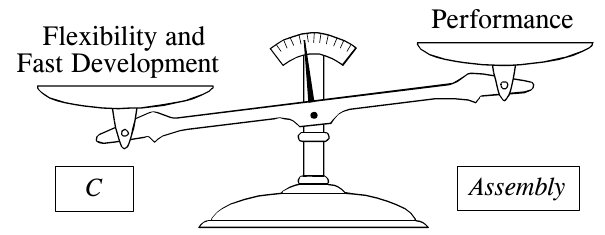
\includegraphics[width=0.504\linewidth,height=0.8\textheight,keepaspectratio]{assets/ch28/fig28-10.png}
\caption*{\textbf{图 28-10　汇编与 C。} C
程序更灵活、开发更快。相比之下，汇编程序往往性能更好：运行更快、占用存储器更少，从而成本更低。
（天平左盘：Flexibility and Fast Development = 灵活性与快速开发，对应
C；右盘：Performance = 性能，对应 Assembly =
汇编。原书图注排在图左侧，裁图时已去掉，译文见上。）}
\end{figure}

哪种语言最适合你的应用？这取决于什么对你更重要。如果你需要灵活性和快速开发，选
C；另一方面，如果你需要尽可能好的性能，就用汇编。如图 28-10
所示，这是一个你不得不做的取舍。下面是一些你应该考虑的事情。

\begin{itemize}
\tightlist
\item
  \textbf{程序有多复杂？} 如果又大又复杂，你大概会想用
  C。如果又小又简单，汇编可能是个好选择。
\item
  \textbf{你是否在逼近 DSP 的最高速度？}
  如果是，汇编能从器件上榨出最后一滴性能。对要求不那么高的应用，汇编没什么优势，你应该考虑用
  C。
\item
  \textbf{有多少程序员一起工作？}
  如果项目大到需要不止一个程序员，就倾向于用
  C，只在时间关键的部分用内嵌汇编。
\item
  \textbf{产品成本和开发成本哪个更重要？}
  如果是产品成本，选汇编；如果是开发成本，选 C。
\item
  \textbf{你的背景是什么？}
  如果你有汇编经验（在其他微处理器上），就为你的 DSP
  选汇编。如果你以前的工作用的是 C，就为你的 DSP 选 C。
\item
  \textbf{DSP 厂商建议你用什么？}
\end{itemize}

最后一项非常重要。假设你问一家 DSP 厂商该用哪种语言，他们告诉你：``C
和汇编都可以用，但我们推荐
C。''你最好听他们的！他们真正的意思是：``我们的 DSP
用汇编编程太难了，你得培训 6 个月才能用。''另一方面，有些 DSP
很容易用汇编编程，例如 Analog Devices
的产品就属于这一类。问问他们的工程师就知道了；他们对此非常自豪。

对 DSP
产品和软件做决定的最好办法之一，是和用过它们的工程师交谈。向厂商要使用其产品的公司作为参考，或者在网上搜索可以发电子邮件联系的人。别害羞；工程师都喜欢对用过的产品发表意见。你去问他们，他们会受宠若惊。

\section{DSP 有多快？}

用 DSP
而不用传统微处理器的首要原因是速度：把采样送进器件、执行所需的数学运算、输出处理后数据的能力。这就引出了一个问题：DSP
有多快？回答这个问题的常用方式是基准测试(benchmark)，即把微处理器的速度表达成一个数的方法。例如，定点系统常用
MIPS（million integer operations per
second，每秒百万次整数运算）来标称。同样，浮点器件可以用 MFLOPS（million
floating point operations per second，每秒百万次浮点运算）来标定。

一百五十年前，英国首相本杰明·迪斯雷利(Benjamin
Disraeli)宣称谎言有三种：谎言、该死的谎言和统计数字。如果迪斯雷利活在今天、和微处理器打交道，他会把基准测试列为第四种。基准测试的想法是提供一个正面对比，表明哪个器件最好。可惜这在实际中常常行不通，因为不同的微处理器擅长不同的领域。想象一下这样问：凯迪拉克和法拉利哪辆车更好？这取决于你要拿它干什么！

电子行业的竞争性加剧了对基准测试的混淆。厂商都想以最好的面貌展示自己的产品，他们会利用测试程序中的任何模糊之处为自己谋利。电子行业有句老话：``写规格书的人能从一个器件上得到的性能，是工程师的两倍。''这些人并没有撒谎，他们只是拿钱来发挥丰富的想象力。基准测试应被看作完成一项复杂任务的工具。如果你不熟悉这个工具的用法，可能会得出错误的结论。更好的办法是去找你打算执行的算法的具体执行速度信息。例如，如果你的应用需要
FIR 滤波器，就去找器件执行这个特定任务所需的确切时钟周期数。

用这种策略，我们来看看在本章重点介绍的 DSP------Analog Devices SHARC
系列------上执行各种算法所需的时间。记住微处理器的速度大约每三年翻一番。这意味着你应特别注意我们在这个例子中使用的方法。实际的数字总在变，每开始一个新项目，你都需要重新计算。在二十一世纪的技术世界里，一眨眼你就过时了！

\begin{figure}[htbp]
\centering
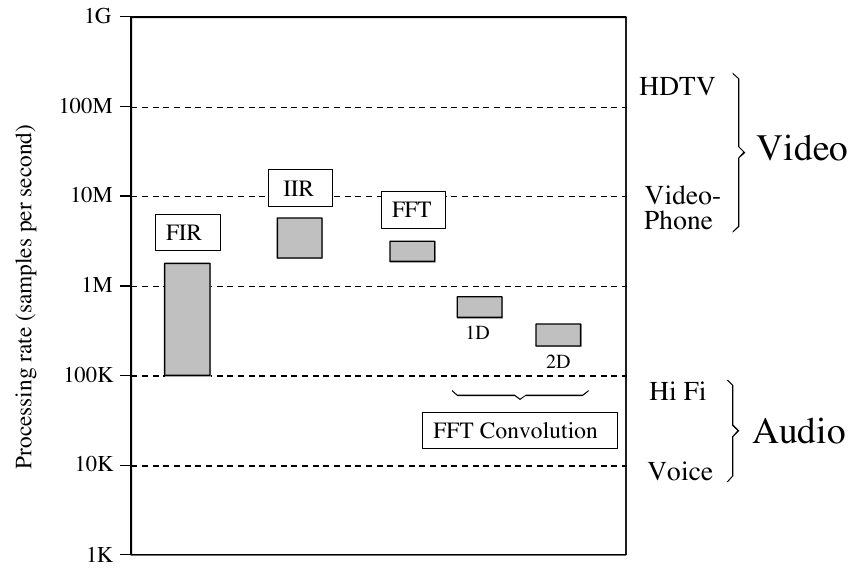
\includegraphics[width=0.717\linewidth,height=0.8\textheight,keepaspectratio]{assets/ch28/fig28-11.png}
\caption*{\textbf{图 28-11　DSP 的速度。} 某个 DSP
算法的吞吐量，可以用时钟频率除以每个采样所需的时钟周期数求得。本图给出了在
40 MHz 时钟下的 SHARC DSP 上执行四种常见算法的吞吐量范围。 （纵轴
Processing rate (samples per second) =
处理速率（采样/秒）；FIR、IIR、FFT、FFT Convolution = FFT 卷积（1D =
一维，2D = 二维）；右侧 Video = 视频（HDTV = 高清电视，Video-Phone =
可视电话），Audio = 音频（Hi Fi = 高保真，Voice = 语音）。）}
\end{figure}

说到理解执行时间，SHARC 系列是最容易打交道的 DSP
之一，因为它能在一个时钟周期内完成一次乘加(multiply-accumulate)运算。由于大多数
FIR 滤波器使用 25 到 400 个系数，处理每个采样相应地需要 25 到 400
个时钟周期。如前所述，实现这种循环效率需要少量开销（预装第一次循环和完成最后一次循环），但循环次数这么多时可以忽略。要得到滤波器的吞吐量，可以用
SHARC 的时钟频率（目前为 40
MHz）除以每个采样所需的时钟周期数。这得到最大 FIR 数据率约为每秒 100k 到
1.6M 个采样。计算不能再简单了！这些 FIR 吞吐量值标在图 28-11 中。

递归滤波器的计算同样简单。典型的 IIR 滤波器使用约 5 到 17
个系数。由于这些循环相对较短，我们再加上少量开销，比如每个采样 3
个周期。这样处理每个数据采样需要 8 到 20 个时钟周期。在 40 MHz
时钟频率下，这给出最大 IIR 吞吐量为每秒 1.8M 到 3.1M 个采样。这些 IIR
值也标在图 28-11 中。

\begin{quote}
\textbf{译注：} 按同样的算法，40 MHz ÷ 20 周期 = 2M，40 MHz ÷ 8 周期 =
5M，应为每秒约 2M 到 5M 个采样；图 28-11 中 IIR 方框的范围（约
2M～5M）也与此相符，原文''1.8M 到 3.1M''疑为笔误。
\end{quote}

接下来是基于快速傅里叶变换的频域技术。FFT 子程序几乎总是由 DSP
厂商提供，这些是用汇编写的高度优化的例程。ADSP-21062 SHARC DSP
的规格书指出，1024 点复数 FFT 需要 18,221 个时钟周期，在 40 MHz 下约
0.46 毫秒。为了计算吞吐量，把它看成每个采样 17.8
个时钟周期更方便。这个''每采样''值随 FFT 长度变化很小。例如，256 点 FFT
每个采样约需 14.2 个时钟周期，4096 点 FFT 每个采样需 21.4
个时钟周期。实数 FFT 比这些复数 FFT 的值快约 40\%。这使得所有 FFT
例程的总体范围约为每个采样 10 到 22 个时钟周期，对应的吞吐量约为每秒
1.8M 到 3.3M 个采样。

\begin{quote}
\textbf{译注：} 40 MHz ÷ 22 = 1.8M，40 MHz ÷ 10 = 4M；原文上限 3.3M
对应的是每采样约 12 个周期（即实数 FFT 的典型值），与''10 到
22''的范围略不一致。
\end{quote}

FFT 卷积是执行 FIR 滤波器的一种快速方法。在典型情况下，从输入中取一段
512 个采样，再补上 512 个零，用 1024 点 FFT
转换成频谱。把这个频谱乘以期望的频率响应后，用 1024 点逆 FFT
回到时域。得到的 1024 个点用重叠相加法与相邻的已处理段合并，产生 512
个输出信号点。

这需要多少时钟周期？每个 512 采样段需要两次 1024 点
FFT，外加少量开销。粗略地说，这大约是一次 512 点 FFT 的五倍。由于实数
FFT 每个采样约需 12 个时钟周期，FFT 卷积大约每个采样 60
个时钟周期就能完成。对 40 MHz 的 2106x SHARC DSP，这相当于约每秒 660k
个采样的数据吞吐量。

注意，这和用常规卷积执行一个 60 系数的 FIR
滤波器差不多。换句话说，如果一个 FIR 滤波器的系数少于 60
个，用标准卷积执行更快；如果多于 60 个，FFT 卷积更快。FFT
卷积的一个关键优点是：执行时间只随系数个数的对数增长。例如，一个 4,096
点的滤波器核，执行时间只比 512 点的长约 30\%。

FFT 卷积也可以用于二维，比如图像处理。例如，假设我们要在频域处理一幅
800×600 像素的图像。首先用零把图像补成 1024×1024。然后对每一行做
FFT，再对得到的每一列做 FFT，就算出了二维频谱。把这个 1024×1024
的频谱乘以期望的频率响应后，做二维逆 FFT：先对每一行做逆
FFT，再对得到的每一列做逆
FFT。把时钟周期数加起来再除以采样数，我们发现整个过程大约每个像素需要
150 个时钟周期。对 40 MHz 的 ADSP-2106x，这相当于约每秒 260k
个采样的数据吞吐量。

比较图 28-11 中的这些不同技术，我们可以得出一个重要的观察：几乎所有 DSP
技术的执行都需要 4 到 400 条指令（在 SHARC
系列中即时钟周期）。对于工作在 40 MHz 的 SHARC
DSP，我们立刻可以断定，视所用算法的复杂程度，它的数据吞吐量在每秒 100k
到 10M 个采样之间。

现在我们知道了 DSP
处理数字化信号能有多快，再把注意力转向另一端：我们需要多快地处理数据？当然，这取决于应用。我们来看两个最常见的应用：音频和视频处理。

音频信号所需的数据率取决于对重现声音质量的要求。在低端，电话质量的语音只需捕获约
100 Hz 到 3.2 kHz 之间的频率，这决定了约每秒 8k
个采样的采样率。相比之下，高保真音乐必须包含人耳听觉的完整范围 20 Hz 到
20 kHz。左右声道常各用 44.1 kHz 的采样率，使完整的高保真信号为每秒 88.2k
个采样。SHARC 系列与这些要求相比如何？如图 28-11
所示，它能轻松处理高保真音频，或同时处理几十路语音信号。

视频信号就是另一回事了；它们需要的数据率约为音频信号的一千倍。低质量视频的一个好例子是可视电话用的
CIF 标准（原文写作 Common Interface Format，通行名称是 Common
Intermediate Format，通用中间格式）。它使用 352×288 像素，每个像素 3
种颜色，每秒 30 帧，总数据率为每秒 910 万个采样。在高质量一端是
HDTV（高清电视），使用 1920×1080 像素，每个像素 3 种颜色，每秒 30
帧，需要每秒超过 1.86 亿个采样的数据率。如图 28-11
所示，这些数据率超出了单个 SHARC DSP
的能力。还有其他应用也需要这么高的数据率，比如雷达、声呐，以及导弹制导等军事用途。

为了处理这些高负荷任务，可以把多个 DSP
组合进一个系统，这叫多处理(multiprocessing)或并行处理(parallel
processing)。SHARC DSP
在设计时就考虑到了这类多处理，并包含了让它尽可能容易实现的特殊功能。例如，把多个
SHARC DSP
的外部总线连在一起不需要外部硬件逻辑；所有总线仲裁逻辑都已包含在每个器件内部。另一种选择是用链路端口(link
port)（4 位并行）把多个处理器以各种配置连接起来。图 28-12 展示了 SHARC
DSP 在多处理系统中的典型排布方式。在图 (a)
中，算法被分解成顺序的步骤，每个处理器以''流水线''的策略执行其中一步。在
(b)
中，处理器通过一个共享的全局存储器交互，经一条并行总线（即外部端口）访问。图
28-13
展示了把大量处理器组合进单个系统的另一种方式：二维或三维''网格(mesh)``。每种配置对特定任务都各有利弊。

\begin{figure}[htbp]
\centering
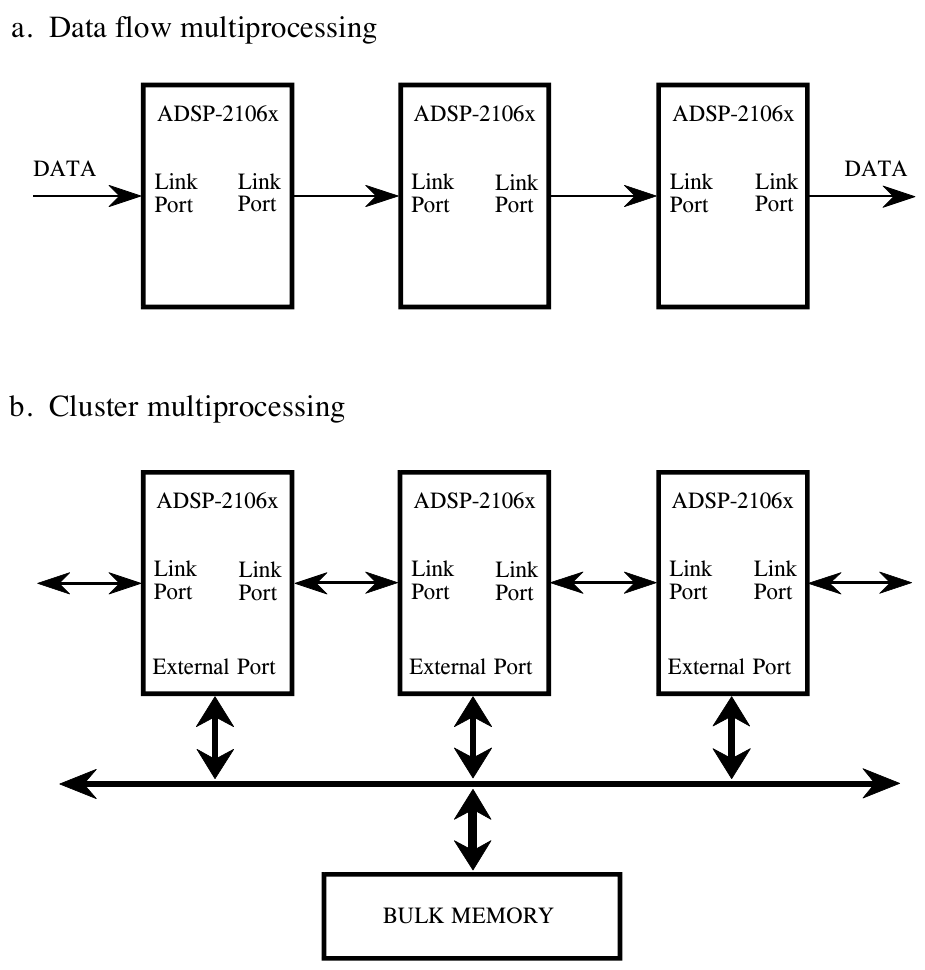
\includegraphics[width=0.771\linewidth,height=0.8\textheight,keepaspectratio]{assets/ch28/fig28-12.png}
\caption*{\textbf{图 28-12　多处理配置。}
多处理器系统通常采用两种方案之一在处理器节点之间通信：(a)
专用的点对点通信通道，或 (b) 经并行总线访问的共享全局存储器。 （a. Data
flow multiprocessing = 数据流多处理；b. Cluster multiprocessing =
集群多处理；ADSP-2106x 为 SHARC 处理器型号，Link Port =
链路端口，External Port = 外部端口，DATA = 数据，BULK MEMORY =
大容量存储器。）}
\end{figure}

\begin{figure}[htbp]
\centering
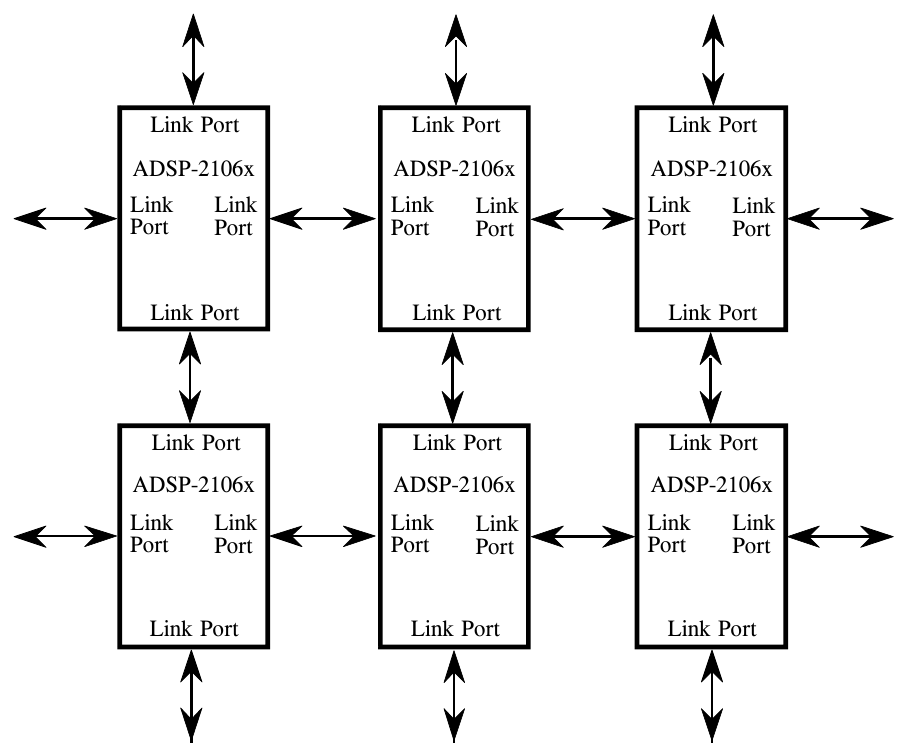
\includegraphics[width=0.754\linewidth,height=0.8\textheight,keepaspectratio]{assets/ch28/fig28-13.png}
\caption*{\textbf{图 28-13　多处理''网格''配置。}
对于雷达成像之类的应用，二维或三维阵列可能是协调大量处理器最有效的方式。
（ADSP-2106x 为 SHARC 处理器型号，Link Port = 链路端口。）}
\end{figure}

为了让程序员的日子好过些，SHARC 系列使用统一的地址空间。这意味着由 32
位地址总线访问的 4 G
字地址空间，被分给协同工作的各个处理器。要把数据从一个处理器传到另一个，只需读写相应的存储单元。其余的事由
SHARC 内部逻辑负责，以高达 240 MB/s（40 MHz
时）的速率在处理器之间传送数据。

\section{数字信号处理器市场}

DSP 市场非常大，而且增长迅速。如图 28-14 所示，到世纪之交它将达到每年约
80～100 亿美元，并以每年 30\%～40\%
的速度增长。推动这一增长的，是对手机、多媒体计算机和高保真音乐重放等更好、更便宜的消费类产品源源不断的需求。这些高收入应用正在塑造这个领域，而利润较低的领域（比如科学仪器）只是顺着技术的浪潮前进。

\begin{figure}[htbp]
\centering
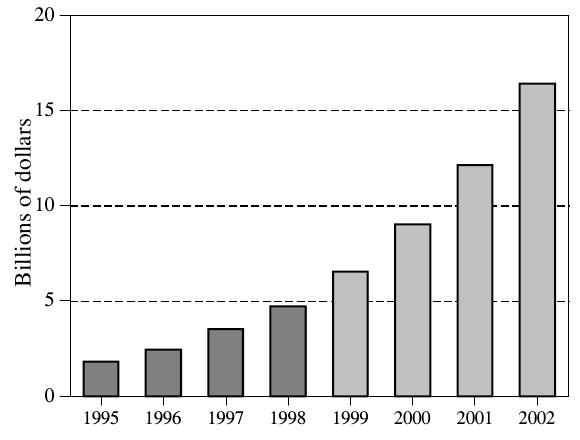
\includegraphics[width=0.483\linewidth,height=0.8\textheight,keepaspectratio]{assets/ch28/fig28-14.png}
\caption*{\textbf{图 28-14　DSP 市场。} 到世纪之交，DSP 市场将达到每年 80～100
亿美元，并以每年约 30\%～40\% 的速度扩张。 （纵轴 Billions of dollars =
十亿美元；横轴为年份
1995～2002。原书图注排在图左侧，裁图时已去掉，译文见上。）}
\end{figure}

DSP
可以以三种形式购买：作为内核(core)、作为处理器(processor)，以及作为板级产品(board
level product)。在 DSP
中，``内核''指处理器中执行关键任务的那部分，包括数据寄存器、乘法器、ALU、地址发生器和程序定序器。完整的处理器需要把内核与存储器和对外接口组合起来。虽然内核和这些外围部分是分开设计的，但它们会制造在同一块硅片上，使处理器成为单个集成电路。

假设你生产手机，想在设计中加入一个 DSP。你大概会想以处理器的形式购买
DSP，也就是一块包含内核、存储器和其他内部功能的集成电路（``芯片''）。例如，SHARC
ADSP-21060 采用''240 引脚公制 PQFP''封装，尺寸只有 35×35×4 mm。要把这块
IC
用进你的产品，你要设计一块印刷电路板，把它焊在你的其他电子器件旁边。这是
DSP 最常见的使用方式。

再假设你所在的公司自己制造集成电路。这时你可能不想要整个处理器，只想要内核的设计。签订相应的许可协议后，你就可以开始制造针对你的特定应用高度定制的芯片。这让你可以灵活地选择包含多少存储器、芯片怎样收发数据、怎样封装等等。这类定制器件是
DSP 市场中日益重要的部分。

最后，有几十家公司出售已经装在印刷电路板上的
DSP。这些板卡有额外的存储器、A/D 和 D/A 转换器、EPROM
插座、同一块板上的多个处理器等功能。虽然有些板卡打算作为独立的计算机使用，但大多数被配置成插到主机（比如个人计算机）上使用。生产这类板卡的公司叫做第三方开发商(Third
Party Developers)。找到它们的最好办法是去问你想用的 DSP 的厂商。看看 DSP
厂商的网站；如果那里找不到名单，就给他们发电子邮件。他们会非常乐意告诉你谁在用他们的产品、怎样联系。

当今（1998
年）的数字信号处理器市场由四家公司主导。下面是名单，以及它们给产品编号的大致方案：

{\def\LTcaptype{none} % do not increment counter
\begin{longtable}[]{@{}lll@{}}
\toprule\noalign{}
公司 & 型号系列 & 类型 \\
\midrule\noalign{}
\endhead
\bottomrule\noalign{}
\endlastfoot
Analog Devices（www.analog.com/dsp） & ADSP-21xx & 16 位定点 \\
& ADSP-21xxx & 32 位浮点与定点 \\
Lucent Technologies（www.lucent.com） & DSP16xxx & 16 位定点 \\
& DSP32xx & 32 位浮点 \\
Motorola（www.mot.com） & DSP561xx & 16 位定点 \\
& DSP560xx & 24 位定点 \\
& DSP96002 & 32 位浮点 \\
Texas Instruments（www.ti.com） & TMS320Cxx & 16 位定点 \\
& TMS320Cxx & 32 位浮点 \\
\end{longtable}
}

\begin{quote}
\textbf{译注：} 这是 1998
年前后的情况，其中几家公司和网址后来都已变化（例如 Lucent
的半导体业务后来拆分为 Agere，Motorola 的半导体部门后来成为
Freescale，再后来并入
NXP）。这条是译者凭一般知识补充的背景，未逐一核实。
\end{quote}

要记住，DSP
与其他微处理器之间的区别并不总是泾渭分明。例如，看看英特尔是怎样描述其奔腾处理器新增的
MMX 技术的：

\begin{quote}
``英特尔的工程师新增了 57
条功能强大的新指令，专门用来高效地操作和处理视频、音频和图形数据。这些指令面向多媒体运算中常见的高度并行、重复性的序列。''
\end{quote}

将来，我们无疑会看到更多类似 DSP
的功能被融入传统的微处理器和微控制器。互联网和其他多媒体应用是推动这些变化的强大动力。这些应用扩张得如此之快，二十年后，数字信号处理器很有可能就成了''传统''微处理器。

怎样跟上这个瞬息万变的领域？最好的办法是阅读报道 DSP
市场的行业期刊，比如 EDN（Electronic Design News，www.ednmag.com）和
ECN（Electronic Component
News，www.ecnmag.com）。这些期刊是免费发放的，包含关于有什么产品、行业走向何方的最新信息。行业期刊是任何认真对待这个领域的人的''必读物''。你还会想加入几家
DSP
厂商的邮件列表，这样能收到新产品公告、价格信息和特别优惠（比如免费软件和低价评估套件）。有些厂商还定期发行通讯。例如，Analog
Devices 每年出版四期《Analog
Dialogue》，刊登关于信号处理当前热点的文章和信息。所有这些资源以及更多资源，都可以通过互联网联系到。先浏览厂商的网站，然后给他们发电子邮件，索取具体信息。
